\section{Propósito y mapa de evidencias}

La pregunta supervisada es cuánto aportan el audio y los géneros a la estimación de
\code{popularity}, un valor histórico entre 0 y 100. La pregunta no supervisada es si
los atributos musicales permiten describir perfiles útiles para explorar el catálogo.
El KPI retrospectivo simula una capacidad de revisión del 10\,\% de la prueba y cuenta
cuántas canciones con \code{popularity >= 70} aparecen en esa lista. El valor real ya
existe en la fuente: el ejercicio no representa una decisión comercial lista para usar.

\begin{table}[htbp]
\centering\small
\begin{tabularx}{\linewidth}{>{\raggedright\arraybackslash}p{0.29\linewidth}X}
\toprule
Artefacto & Uso para Ignacio, César y el notebook integrador \\
\midrule
\path{docs/ea2/protocolo_comun.md} & Definiciones compartidas de datos, particiones, modelos y métricas. \\
\path{notebooks/04a_modeling_lucas.ipynb} & Cálculo reproducible, salidas, figuras e interpretación del trabajo de Lucas. \\
\path{src/spotify_popularity/modeling/protocol.py} & Funciones de partición, codificación, pipelines y métricas. \\
\path{docs/ea2/lucas.md} & Alcance individual y reproducción desde instalación limpia. \\
Este informe & Síntesis para revisión cruzada; las cifras oficiales del equipo se recalculan en el notebook 05. \\
\bottomrule
\end{tabularx}
\caption{Función de cada artefacto en el traspaso.}
\label{tab:mapa}
\end{table}

\section{Metodología, fuente y preparación}

El trabajo sigue CRISP-DM de manera verificable: pregunta y KPI para la
\emph{comprensión del negocio}; controles de la fuente y hallazgos de EP1 para la
\emph{comprensión de datos}; deduplicación y codificación para la \emph{preparación};
Ridge, árbol y K-Means para \emph{modelamiento}; pruebas, segmentos, ranking y
sensibilidades para \emph{evaluación}; notebook e informe para la entrega académica,
sin despliegue operativo. La evaluación retroalimenta la definición de uso: los
errores extremos impiden recomendar decisiones automáticas.

La fuente inmutable es \path{data/raw/Spotify_Tracks_Dataset.csv}, con SHA-256:

{\footnotesize\ttfamily\noindent b202fa49909b2d5cef71a04b1d21243cfeb36414535f2ca9272aa646721177bd\par}
De 114.000 filas se retiró una inválida y se consolidaron 24.259 repeticiones de
\code{track_id}; el procesado tiene 89.740 canciones únicas, 20 columnas y cero
faltantes. La popularidad queda en 0--100. EP1 encontró 10,47\,\% de ceros,
3,48\,\% de canciones con popularidad al menos 70 y asociaciones acústicas
individuales débiles. La fuente aportaba exactamente 1.000 filas por género antes
de consolidar duplicados; sus frecuencias no representan el catálogo natural.

\begin{figure}[htbp]
\centering
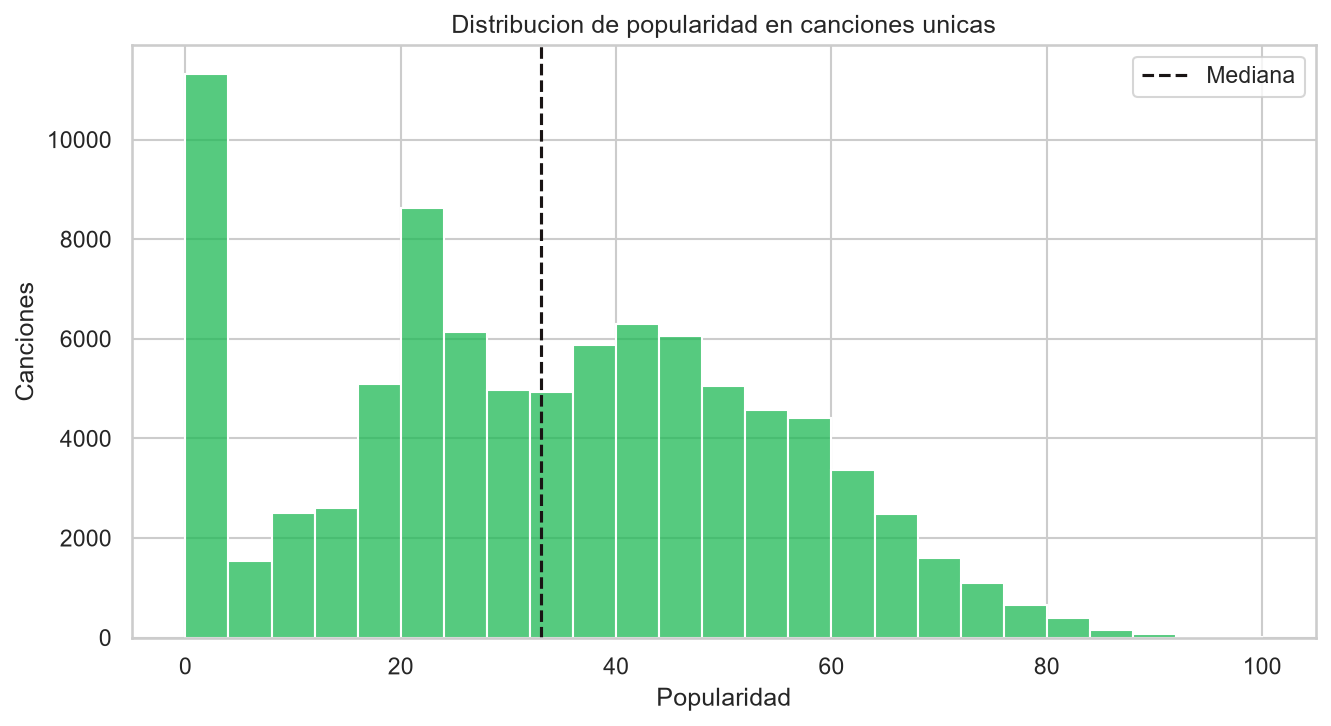
\includegraphics[width=0.81\linewidth]{05_processed_popularity_distribution.png}
\caption{Distribución de popularidad del procesado, proveniente del EDA de EP1. Los extremos justifican la referencia mediana y el diagnóstico por rangos.}
\label{fig:target}
\end{figure}

\begin{figure}[htbp]
\centering
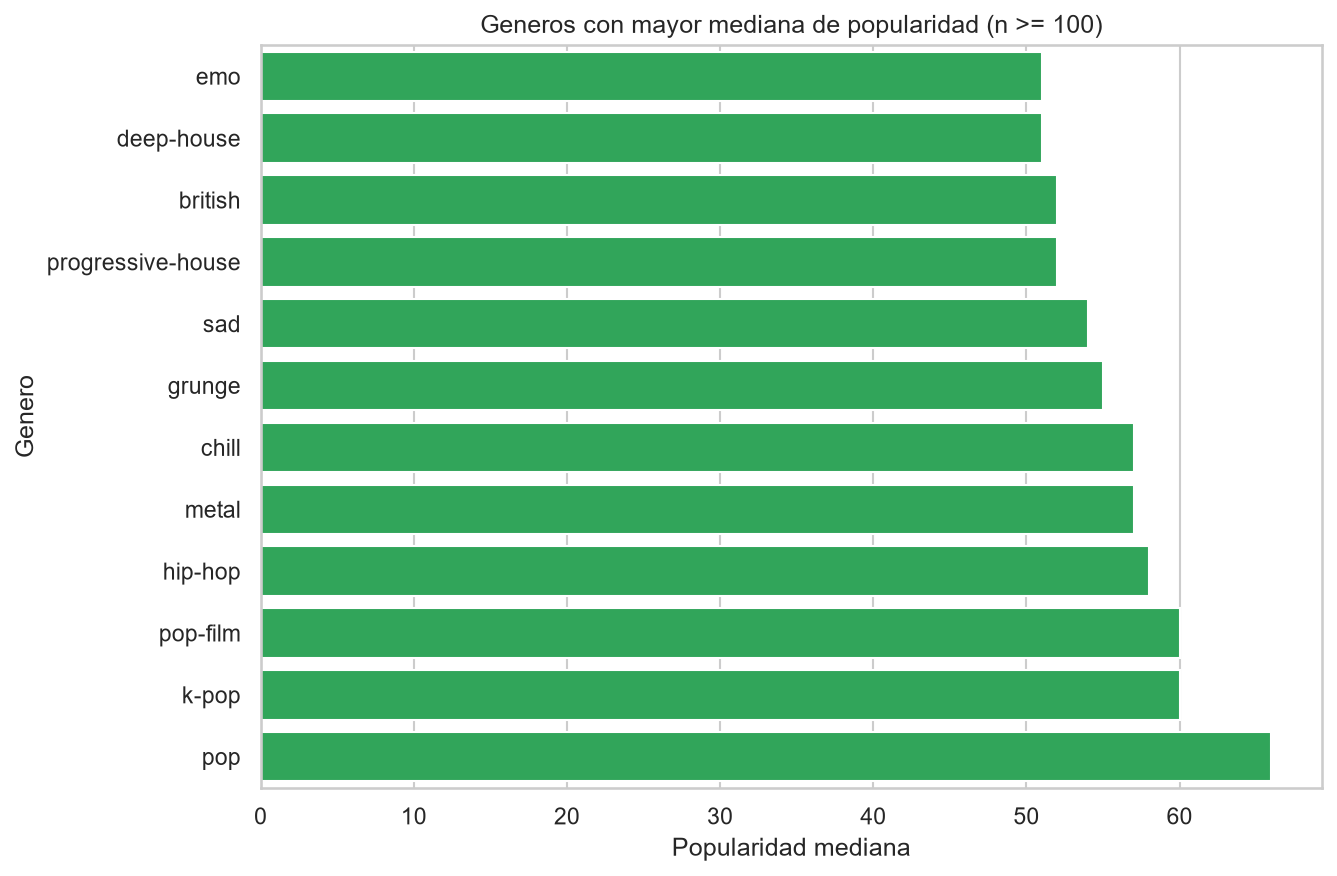
\includegraphics[width=0.81\linewidth]{09_genre_popularity_summary.png}
\caption{Resumen descriptivo por género elaborado en EP1. Su lectura está condicionada por el diseño de muestreo.}
\label{fig:genre-eda}
\end{figure}

\subsection{Partición común y prevención de fuga}

Se ordenaron los \code{track_id} únicos y se aplicó \code{train_test_split} con
\code{test_size=0.20}, semilla 42 y mezcla aleatoria. Quedaron 71.792 canciones
de entrenamiento y 17.948 de prueba. Del entrenamiento se apartó un 20\,\%
adicional: 57.433 para ajustar candidatos y 14.359 para validarlos. La huella
SHA-256 de los IDs ordenados de la prueba aleatoria es:

{\footnotesize\ttfamily\noindent 7270ff57b6fb81215fba2f834942d194183e3854ccac935a65e5a03f7888b318\par}
Los tres integrantes deben usar esos mismos IDs para la comparación principal.

El objetivo, \code{track_id}, nombres, álbum y artistas no entraron como predictores.
Las diez columnas numéricas fueron \code{duration_ms}, \code{danceability},
\code{energy}, \code{loudness}, \code{speechiness}, \code{acousticness},
\code{instrumentalness}, \code{liveness}, \code{valence} y \code{tempo}. Las
cuatro categóricas fueron \code{key}, \code{mode}, \code{time_signature} y
\code{explicit}. \code{track_genres} se separó por \code{|} y se codificó como
multietiqueta. Escalado, one-hot y codificación de géneros se ajustaron dentro de
cada pipeline usando solo la partición de entrenamiento correspondiente; las
etiquetas no vistas se ignoran.
